\begin{figure*}[t]
    \centering
    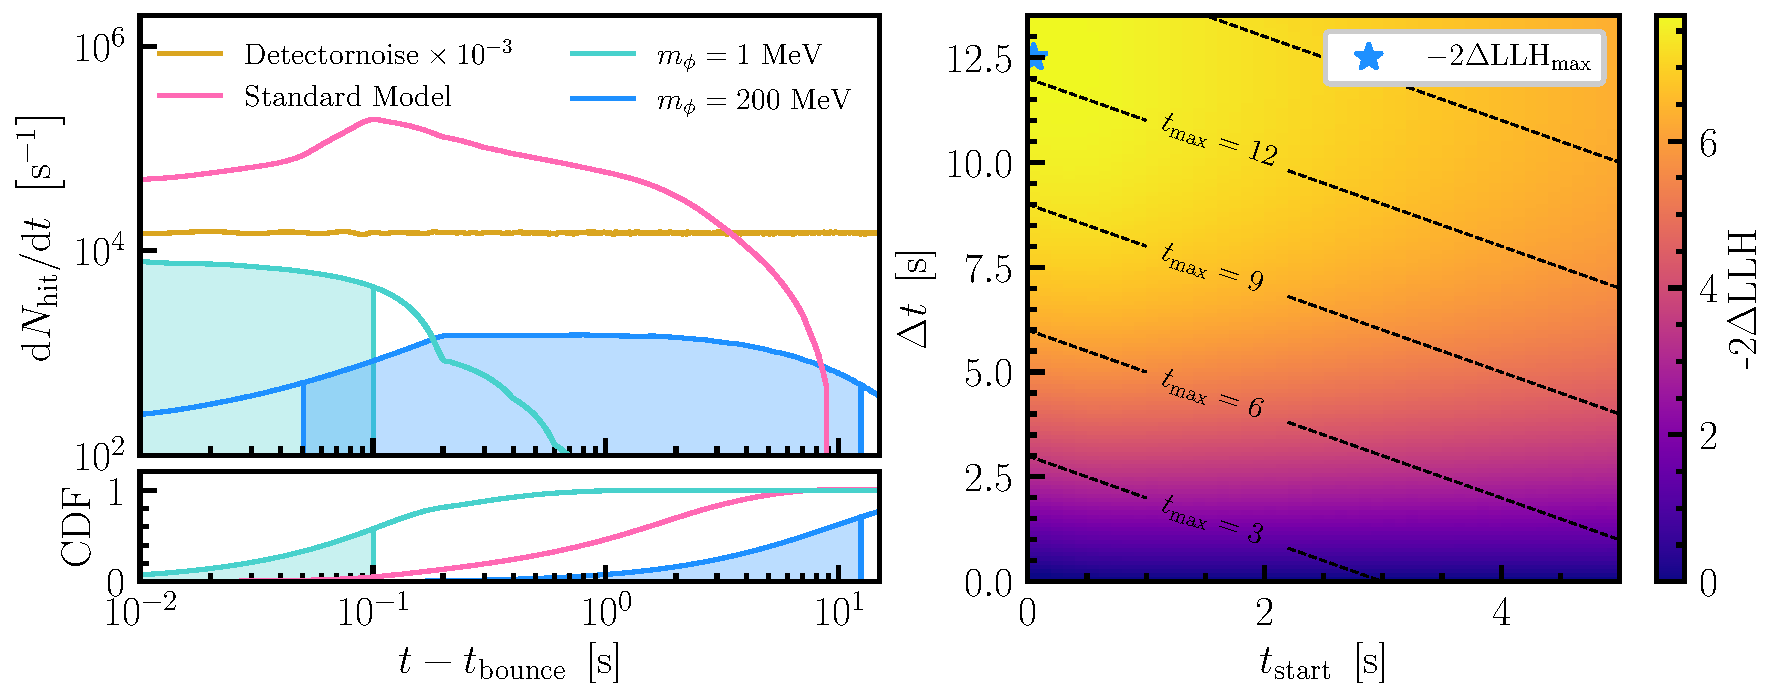
\includegraphics[width=0.95\textwidth]{figures/hits_and_likelihood.pdf}
    \caption{\textbf{\textit{Timing profile of hits and test statistic as a function of the timing window.}}
    The hit rate from the SM neutrino flux peaks at around 0.1~s, coinciding with the peak emission of $\bar{\nu}_{e}$ from the SN.
    The shaded regions correspond to the timing windows that give peak sensitivity to the particular model.
    In the right panel, we show the test statistic as a function of the starting time and length of the window.
    The relatively broad distribution of high test-statistic values shows that this analysis technique does not require extremely precise reconstruction of the $t_{\mathrm{bounce}}$.
    These are the same points in the parameter space as Fig.~\ref{fig:fluxes}.
    }
    \label{fig:hits_and_likelihood}
\end{figure*}
\
\textbf{\textit{Detector Response and Statistical Treatment}}---The IceCube Neutrino Observatory comprises 5,160 light-detecting digital optical modules (DOMs) buried in a cubic kilometer of the deep, transparent Antarctic ice sheet.
When neutrinos interact within or near the detector, the charged by-products emit photons that the DOMs can detect.
The DOMs are arranged on 86 strings of 60 DOMs with an inter-string distance between 70~m and 125~m.
This enables IceCube to resolve individual neutrinos with energies approximately ranging between a few GeV and a few PeV.
The neutrinos produced by SNe are far below this threshold, and the neutrinos cannot be individually resolved; however, the immense number of neutrinos produced in an SN increases the single-photon rate of the detector.
This dramatic increase in the rate of photons can be distinguished from the background caused by dark noise and radioactive activity in the DOM glass to enable the detection of galactic CCSNe events~\cite{Griswold:2023iwz}.

New neutrino physics will affect the development of an SN and distort the temporal structure of the photon signal seen in the IceCube detector.
Thus, one may look for excess events in certain time intervals as evidence of this new physics.
In this work, we simulate the light curve produced by a standard SN with a progenitor mass of $8.8~M_{\odot}$ and those produced by different BSM scenarios aforementioned; see the left-hand panel of Fig.~\ref{fig:hits_and_likelihood} for light curves of the same two benchmarks discussed above.
Since more than 93\% of the photons detected in IceCube originate in inverse beta decay interactions, the SM-only event rate peaks at around 0.1~s.
BSM scenarios, on the other hand, can give rise to an early or delayed signal depending on the particulars of the model.
In essence, Majorons can be generated before the peak of SM $\bar{\nu}_{e}$ flux and as light majorons can travel nearly relativistically, they can escape the SN with negligible time-delay then decay to an all-flavor flux of neutrinos, producing early $\bar{\nu}_{e}$ fluxes before the SM case.
The higher-mass majorons, on the other hand acquire a time decay from traveling sub-luminally and at a large detour, thus producing a later signal with sizable time delay.
We use the \texttt{ASTERIA}~\cite{spencer_griswold_2020_3926835} package to simulate the detector response to the different SNe scenarios and the thermal and radioactive noise in the DOMs.
 This package simulates light yields from coherent $\nu_{e}$ scattering off electrons in the ice, inverse beta decay of $\bar{\nu}_{e}$ on nuclei in the ice, and charged- and neutral-current interactions for $\nu_{\alpha}$.
In order to interface to this package, we use \texttt{SNEWPY}~\cite{SNEWS:2021ewj} package and, in particular, the \texttt{ParametrizedFlux} object.
In addition to photons produced in neutrino interactions, this package also simulates photons from thermal noise in the IceCube PMTs and from radioactive decay in the pressure glass housing.

With the number of hits in the detector from noise, SM-only scenarios, and BSM scenarios as a function of time, we can then quantify the probability of seeing a certain number of hits in a given time window with:
\begin{equation}
    -2\Delta\mathrm{LLH} = 2 \left[N_{\mathrm{exp.}} - N_{\mathrm{obs.}} + N_{\mathrm{obs.}}\log\left(\frac{N_{\mathrm{obs.}}}{N_{\mathrm{exp.}}}\right)\right].
    % -2\Delta\mathrm{LLH}(t_{\mathrm{start}}, \Delta t) = 2 \left[N_{\mathrm{exp.}} - N_{\mathrm{obs.}} + N_{\mathrm{obs.}}\log\left(\frac{N_{\mathrm{obs.}}}{N_{\mathrm{exp.}}}\right)\right].
\end{equation}
where $N_{\mathrm{obs.}}$ is the number of photons seen in the detector in the given time and $N_{\mathrm{exp.}}$ is the number of photons expected from a particular BSM hypothesis.
In the right-hand panel of Fig.~\ref{fig:hits_and_likelihood}, we show the likelihood space as a function of the time at which the time range begins, $t_{\mathrm{start}}$ and the duration of the time range, $\Delta t$ for an example BSM hypothesis.

For each physics hypothesis, we then select the time range that maximizes the test statistic and use that maximal test statistic value. The optimal ranges for each physics hypothesis are shown by the shaded regions in the left panel of Fig.~\ref{fig:hits_and_likelihood}, which is around $\unit[0.1]{s}$ ($\unit[10]{s}$) for the light (heavy) benchmark case, consistent with its time spread of $\bar{\nu}_e$ flux produced. Furthermore, the test statistic value relative to the SM-only hypothesis is shown in the right-hand panel of Fig.~\ref{fig:hits_and_likelihood}.
The distribution of test-statistic values is not sharply peaked, and thus, this analysis retains much of its sensitivity even with errors on the reconstruction of $t_{\mathrm{bounce}}\sim\mathcal{O}\left(10^{-3}~\mathrm{s}\right)$ \cite{Halzen_2009}.